%\documentclass[10pt, xcolor=x11names, compress]{beamer}
\documentclass[10pt, xcolor=x11names, compress, handout]{beamer}

\usetheme{progressbar}
%\usecolortheme[named=Purple4]{structure}
\progressbaroptions{headline=sections,titlepage=normal,frametitle=normal}

\setbeamertemplate{navigation symbols}{}

\usepackage{iwona} 

\usepackage{alltt}
\usepackage{amsmath,amsfonts, amssymb, amscd}
\usepackage{hyperref}
\usepackage{setspace}
\usepackage{wasysym}
\usepackage{ulem}

\usepackage{calc}
\usepackage[overlay,absolute]{textpos}
\TPGrid[5mm,5mm]{20}{20}


\renewcommand{\Re}{\operatorname{Re}}
\renewcommand{\Im}{\operatorname{Im}}
\newcommand{\debye}{\operatorname{debye}}

\newcommand{\chik}{$\chi(k)$}
\newcommand{\chir}{$|\tilde{\chi}(R)|$}


\newcommand{\file}[1]{{\color{Firebrick4}\texttt{`#1'}}}
\newcommand{\multiple}{{\color{Orange3}\textsl{multiple}}}


\newcommand{\atoms}  {{\color{DarkOrchid4}\textsc{atoms}}}
\newcommand{\feff}   {{\color{DarkOrchid4}\textsc{feff}}}
\newcommand{\ifeffit}{{\color{DarkOrchid4}\textsc{ifeffit}}}
\newcommand{\athena} {{\color{DarkOrchid4}\textsc{athena}}}
\newcommand{\artemis}{{\color{DarkOrchid4}\textsc{artemis}}}

\newcommand{\ybco}{YBa$_2$Cu$_3$O$_7$}
\newcommand{\eto}{EuTiO$_3$}

\renewenvironment<>{center}
{\begin{actionenv}#1\begin{originalcenter}}
{\end{originalcenter}\end{actionenv}}



\mode<presentation>
%\mode<beamer>

\title{Understanding self-absorption in fluorescence XAS}

\author{Bruce Ravel}
\institute[NIST]{Synchrotron Methods Group, Materials Measurement Science Division\\%
  Materials Measurement Laboratory\\%
  National Institute of Standards and Technology\\%
  \&\\%
  Local Contact, Beamline X23A2\\%
  National Synchrotron Light Source\\~}



\date[NSLS2010]{Advanced EXAFS Data Analysis workshop 2011\\
  Universiteit Gent, January 12--14, 2011}


\begin{document}
\begin{frame}
  \titlepage
\end{frame}

\begin{frame}
  \frametitle{Copyright}
  \tiny

  This document is copyright \copyright 2007-2010 Bruce Ravel.

  \begin{center}
    
\includegraphics[width=1.0cm]{images/somerights20}
  \end{center}

  This work is licensed under the Creative Commons
  Attribution-ShareAlike License.  To view a copy of this license,
  visit \href{http://creativecommons.org/licenses/by-sa/3.0/}
  {\color{Purple4}\texttt{http://creativecommons.org/licenses/by-sa/3.0/}}
  or send a letter to Creative Commons, 559 Nathan Abbott Way,
  Stanford, California 94305, USA.

  \begin{description}
  \item[You are free:] %
    \begin{itemize}
    \item \textbf{to Share} --- to copy, distribute, and transmit the work
    \item \textbf{to Remix} --- to adapt the work
    \end{itemize}
  \item[Under the following conditions:] %
    \begin{itemize}
    \item Attribution. You must attribute the work in the manner
      specified by the author or licensor (but not in any way that
      suggests that they endorse you or your use of the work).
    \item Share Alike. If you alter, transform, or build upon this
      work, you may distribute the resulting work only under the same,
      similar or a compatible license.
    \item Any of these conditions can be waived if you get permission
      from the author.
    \end{itemize}
  \end{description}
  \begin{itemize}
  \item For any reuse or distribution, you must make clear to others
    the license terms of this work. The best way to do this is with a
    link to the URL for this document.
  \item Any of the above conditions can be waived if you get
    permission from the copyright holder.
  \item Nothing in this license impairs or restricts the author's
    moral rights.
  \end{itemize}

  Your fair dealing and other rights are in no way affected by the
  above.  This is a human-readable summary of the Legal Code (the full
  license).


\end{frame}

%%% Local Variables:
%%% mode: latex
%%% TeX-master: "pimst2"
%%% End:


%\mode<handout>{\frame{\tableofcontents}}

%% \section*{Outline}
%% \begin{frame}
%%   \tableofcontents
%% \end{frame}


\section[Introduction]{Introduction}
\begin{frame}
  
  Self-absorption is a distortion to the XAS spectrum due to the
  variation in penetration depth into the sample as the energy is
  scanned through the edge and the fine structure.

  \frametitle{Introduction}
  \begin{block}{Nomenclature}
    \textit{Over-absorption} is another term used for the same physical
    phenomenon.
  \end{block}

  \begin{block}{No dependence on detector type}
    Self-absorption cannot be corrected by using a ``better''
    detector.  Be aware, though, that self-absorption and
    \textit{deat-time} have similar impacts on the XAS.
  \end{block}
\end{frame}

\begin{frame}
  \frametitle{Math}

  \small
  \begin{columns}
    \begin{column}{0.35\linewidth}
      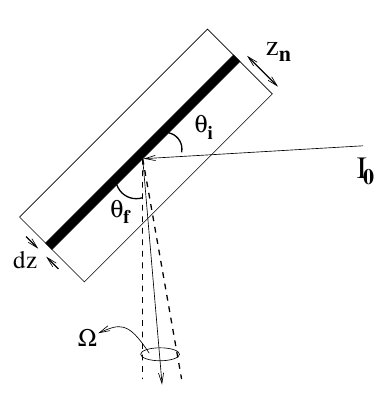
\includegraphics[width=\linewidth]{images/schematic.png}
    \end{column}
    \begin{column}{0.65\linewidth}
      Radiation of intensity $I_0(E)$ impinges on a sample of total
      thickness $z_s$ at an angle $\theta_i$ from the surface. The
      fluorescence radiation is detected with a detector subtending a solid
      angle $\Omega$ centered at an angle $\theta_f$ with the surface.

      \smallskip
      
      The fluorescence intensity $I_f$ due to the edge of interest coming
      from a slice of sample of width $dz$ at depth $z_n$ is given by
    \end{column}
  \end{columns}

  \begin{equation}
    \scriptsize
    \label{eq:dz}
    I_f(z_n)dz_n = \frac{\Omega}{4\pi} I_0\,\exp\big(-\mu_t(E)z_n/\sin(\theta_i)\big)
    \,\epsilon_f(E)\,\mu_e(E) \frac{dz}{\sin(\theta_i)}\,
    \exp\big(-\mu_t(E_f)z_n/\sin(\theta_f)\big)
  \end{equation}

  \begin{tabular}{clcl}
    $\mu_t$ & absorption of entire sample &  $E_f$ & fluorescence energy \\
    $\mu_e$ & absorption of absorber &  $\epsilon_f$ & fluorescence probability \\
    $\mu_b$ & absorption of everything but the absorber &   & \\
    $\mu_t$ & $=\mu_e+\mu_b$ &   & \\
  \end{tabular}
\end{frame}

\begin{frame}
  \frametitle{More math}
  The get the fluorescence from the entire depth of the sample, we
  integrate the expression for $I_f$:
  \begin{equation}
    \label{eq:integ}
    \int_0^{z_s} I_f(z_n) dz_n = I_f(E)
  \end{equation}
  Now do a bunch of math, finally assuming that the sample is
  infinitely thick.  This eventually yields:
  \begin{equation}
    \label{eq:result}
    I_f(E) = I_0(E)\,\frac{\Omega}{4\pi}
    \Bigg[
    \frac{\alert{\mu_e(E)}}
    {\alert{\mu_e(E)}+{\color{Blue4}\mu_b(E)}+\mu_t(E_f)
      \cdot\frac{\sin(\theta_i)}{\color{Green4}\sin(\theta_f)}}
    \Bigg]
  \end{equation}
  \begin{center}
    New we see \alert{the problem}!
  \end{center}
\end{frame}

\begin{frame}
  \frametitle{The consequences of self-absorption}
  \begin{enumerate}
  \item Incorrect XANES peak sizes
  \item Attenuated EXAFS amplitude
  \item Uncertainty in determination of coordination number
  \item Bad standard for linear combination analysis
  \item Bad standard for PCA target transform
  \end{enumerate}
\end{frame}

\begin{frame}
  \frametitle{Avoiding self-absorption}
  \begin{description}[Dilution]
  \item[Do transmission] This is certainly the simplest option!
  \item[Dilution] Making the absorber dilute in your sample makes the
    ${\color{Blue4}\mu_b(E)}$ term dominate the denominator. For solid
    samples, this \textit{requires} that grains be small compared to
    an absorption length.
  \item[Glancing exit angle] Measuring the photons that exit the
    sample at a shallow angle makes the $\color{Green4}\sin(\theta_f)$
    term small, causing the $\mu_t(E_f)$ term dominate the denominator.
  \item[Thin sample] An assumption of a thick sample leads to
    Eq.~\ref{eq:result}.  Make the sample thin compared to an
    absorption length to minimize self-absorption.
  \end{description}
  \begin{alertblock}{However...}
    You cannot always avoid a fluorescence experiment on an unsuitable
    sample. $\ddot\frown$
  \end{alertblock}
\end{frame}

\section{Alloy}
\begin{frame}
  \frametitle{Iron/gallium alloy}
  \begin{columns}
    \begin{column}{0.5\linewidth}
      I was once asked to do some work on an Fe/Ga alloy.  I was given
      a slice taken from a single crystal boule that had been drawn
      out of a melt.  The sample was about the size of a watch battery
      and \textit{I had to give it back undamaged!}

      \medskip

      The sample stoichiometry was Fe$_{72.74}$Ga$_{27.26}$.  The Fe K
      edge data were severely attenutated.
    \end{column}
    \begin{column}{0.5\linewidth}
      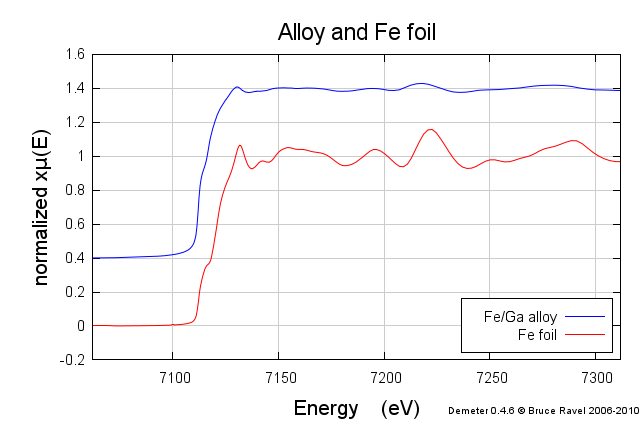
\includegraphics[width=\linewidth]{images/alloy_foil.png}
    \end{column}
  \end{columns}

  \bigskip

  The alloy is still BCC, but the data are, unsurprisingly, severely
  attenuated.
\end{frame}

\begin{frame}
  \frametitle{Correction}
  Applying the correction to the XANES data results in the following:

  \bigskip

  \begin{columns}
    \begin{column}{0.33\linewidth}
      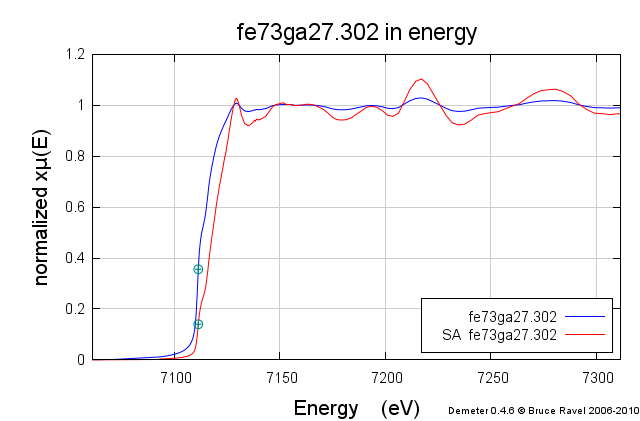
\includegraphics[width=\linewidth]{images/fega_mu.png}
    \end{column}
    \begin{column}{0.33\linewidth}
      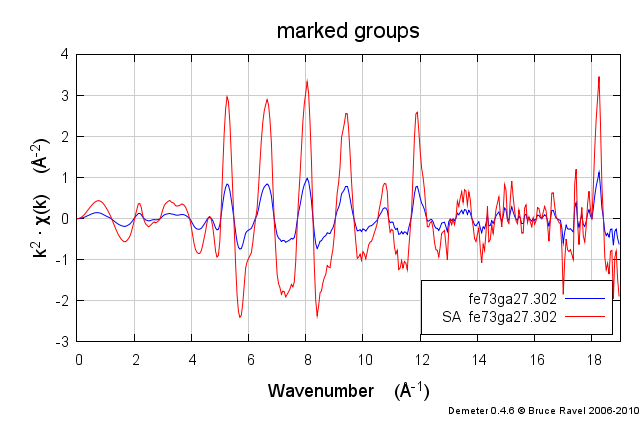
\includegraphics[width=\linewidth]{images/fega_chik.png}
    \end{column}
    \begin{column}{0.33\linewidth}
      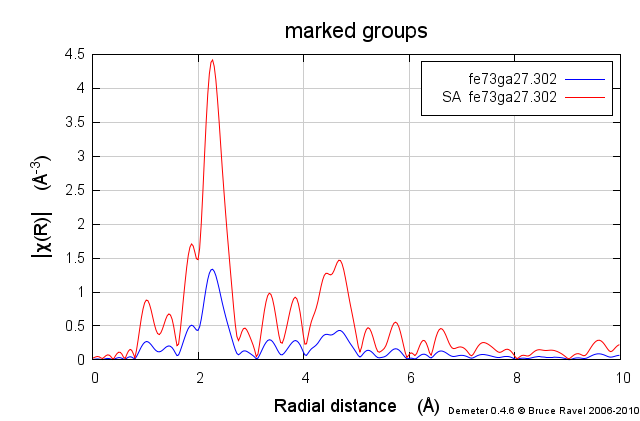
\includegraphics[width=\linewidth]{images/fega_chir.png}
    \end{column}
  \end{columns}

  \bigskip

  These data can be analyzed with a more accurate assessment of
  coordination number.  Some systematic uncertainty remains, but it's
  an improvment on the raw data.

  \bigskip

  \begin{exampleblock}{}
    In this case, we could accurately apply a correction because we
    knew the stoichiometry of every part of the sample interacting
    with the beam.
  \end{exampleblock}

\end{frame}


\section{Solution}
\begin{frame}
  \frametitle{Ammonium sulfate in water}
    \small
  
  \begin{columns}
    \begin{column}{0.5\linewidth}
      Here are some data on various samples of (NH$_4$)$_2$SO$_4$
      dissolved in water.  The samples --- with concetrations of
      0.1\,M, 0.47\,M, and 0.94\,M --- show increasing attenuation of
      the white line.

      \smallskip

      The correction requires the formula of the sample \textbf{and}
      its matrix.
    \end{column}
    \begin{column}{0.5\linewidth}
      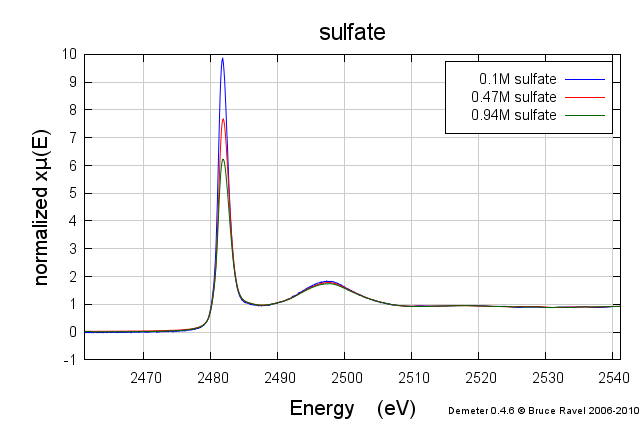
\includegraphics[width=\linewidth]{images/sulfate.png}
    \end{column}
  \end{columns}
  \begin{center}
    \begin{tabular}{r@{~=~}l}
      1 amu & $1.6605\times10^{-27}$ kg \\
      1 mole & $6.0221\times10^{23}$ particles \\
      1 H$_2$O molecule & 18 amu  = $2.988 \times 10^{-26}$ kg \\
      1 mole of water & 0.01800 kg \\
      1 liter of water & 1 kg water \\
      1 liter &  55.6 moles
    \end{tabular}
  \end{center}

  Well ... adjusted for the density change upon adding the solute,
  there are about 54.8 moles of water in the solution.

  \medskip

  The formula for an $\eta$ molar solution is
  \alert{$\big((NH_4)_2SO_4\big)_\eta(H_2O)_{54.8}$}
\end{frame}

\begin{frame}
  \frametitle{Correcting the solutions data}
  \begin{columns}
    \begin{column}{0.5\linewidth}
      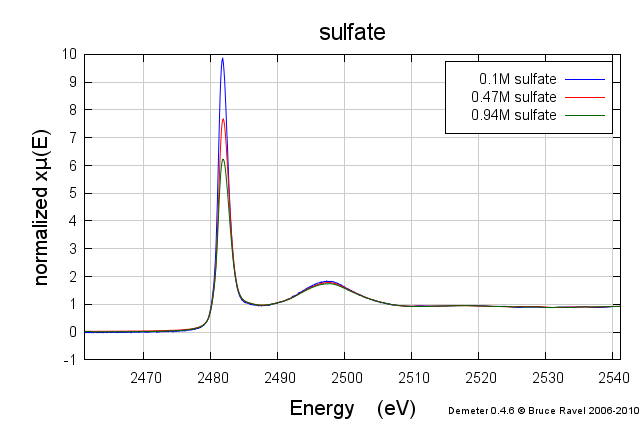
\includegraphics[width=\linewidth]{images/sulfate.png}      
    \end{column}
    \begin{column}{0.5\linewidth}
      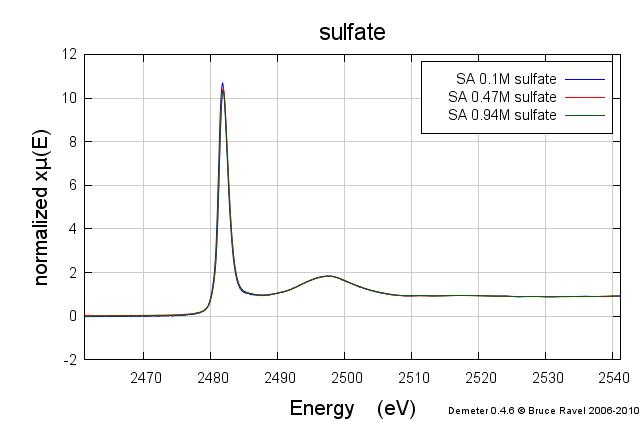
\includegraphics[width=\linewidth]{images/sulfate_sa.png}      
    \end{column}
  \end{columns}
  \begin{center}
    Yay!
  \end{center}

  \begin{exampleblock}{}
    In this case, we know that the correction has been applied
    properly because all three concentrations give the same corrected
    spectrum --- as we reasonably expect.

    \medskip

    We also know that the sample is very heterogeneous, since it is a
    solution.
  \end{exampleblock}

\end{frame}


\section{Ceramic}
\begin{frame}
  \frametitle{Actinide containment ceramics}
  
  CaZrTi$_2$O$_7$ is a model system for actinide containment
  \begin{itemize}
  \item Immobile, stable, self-shielding
  \item $\alpha$ decay induces amorphization of the zirconolite
    structure.  These defects lead to a loss of stability
  \item Looking for a material that can withstand $\alpha$ damage
    without loosing integrity as a containment matrix
  \end{itemize}

  \begin{columns}
    \begin{column}{0.4\linewidth}
      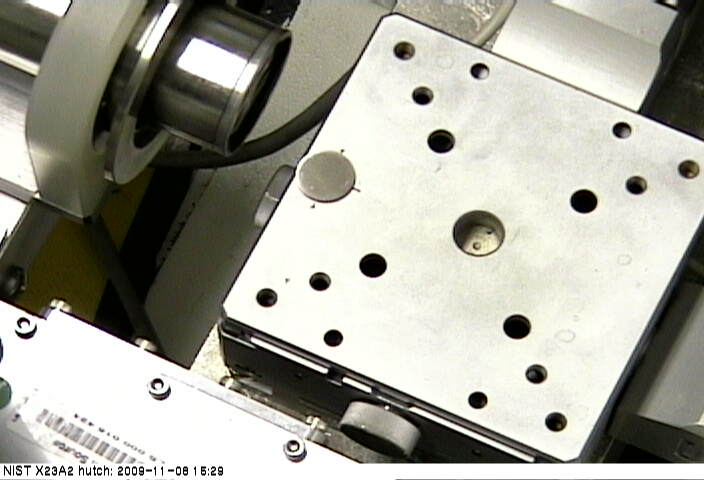
\includegraphics[width=\linewidth]{images/tilt_stage.jpg}
    \end{column}
    \begin{column}{0.6\linewidth}
      The samples are in the form of sintered, \alert{polished}
      pellets.
      \begin{enumerate}
      \item Pristine material
      \item Bombarded with high energy Kr ions to simulate $\alpha$
        damage
      \end{enumerate}
      The samples are measured at glancing angle to isolate the
      1\,$\mu$m thick damaged layer.
    \end{column}
  \end{columns}
\end{frame}

\begin{frame}
  \frametitle{Raw fluorescence data}

  Titanium K-edge spectra can be categorized according to the height
  and position of the 1s-3d peak before the main edge.

  \begin{columns}
    \begin{column}{0.5\linewidth}
      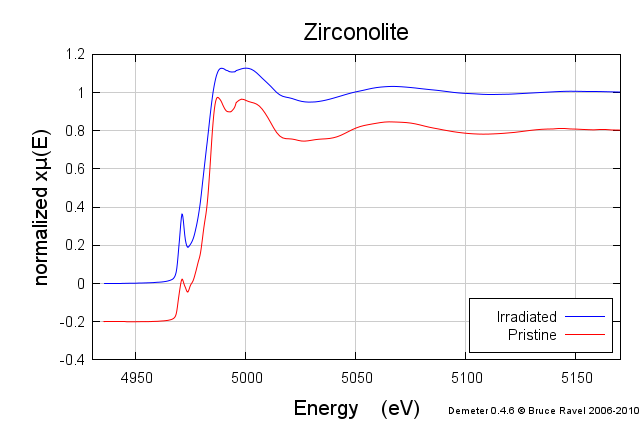
\includegraphics[width=\linewidth]{images/pristine_irrad.png}
    \end{column}
    \begin{column}{0.5\linewidth}
      \begin{center}
        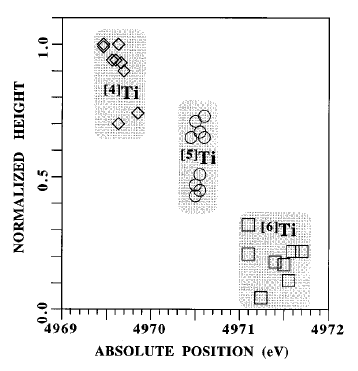
\includegraphics[width=0.8\linewidth]{images/farges.png}
      \end{center}
    \end{column}
  \end{columns}

  \smallskip

  However, a proper assessment of peak height requires a
  self-absorption correction!

  \begin{textblock*}{0.5\linewidth}(0pt,19.5\TPVertModule)
    \tiny%
    F.~Farges, G.E.~Brown, Jr., and J.J.~Rehr, PRB \textbf{56}:4,
    (1997) 1809
    \href{http://dx.doi.org/10.1103/PhysRevB.56.1809}
    {\color{Blue2}doi:10.1103/PhysRevB.56.1809}
  \end{textblock*}
\end{frame}

\begin{frame}
  \frametitle{Correction strategy}
  \small
  First collect data in transmission on a powdered, pristine sample.
  Then collect data in fluorescence on the sintered, pristine sample
  in the same geometry required for measuring the damaged layer of the
  irradiated sample.  Find correction parameters which make the two
  pristine samples the same.
  \begin{columns}
    \begin{column}{0.5\linewidth}
      \begin{center}
        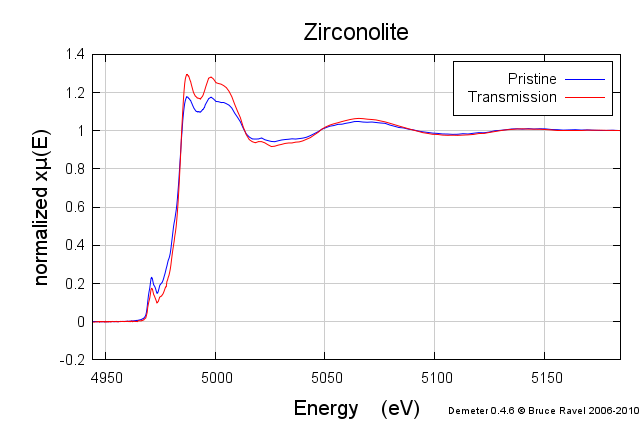
\includegraphics[width=0.8\linewidth]{images/pristine.png}\\
        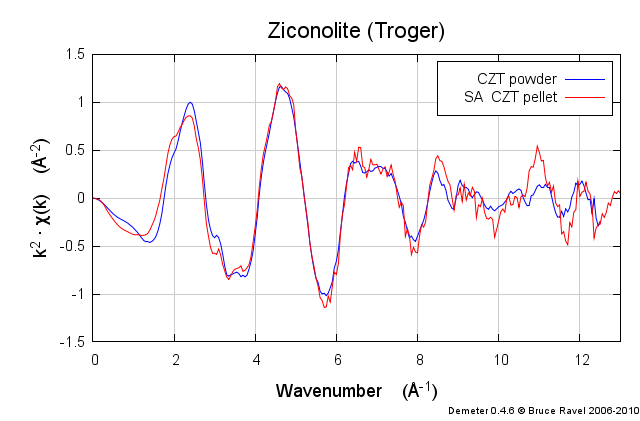
\includegraphics[width=0.8\linewidth]{images/zirconolite_chik.png}
      \end{center}
    \end{column}
    \begin{column}{0.5\linewidth}
      \begin{center}
        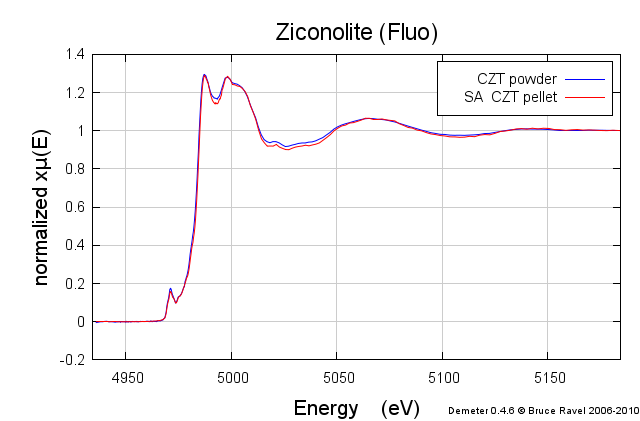
\includegraphics[width=0.8\linewidth]{images/zirconolite_mu.png}\\
        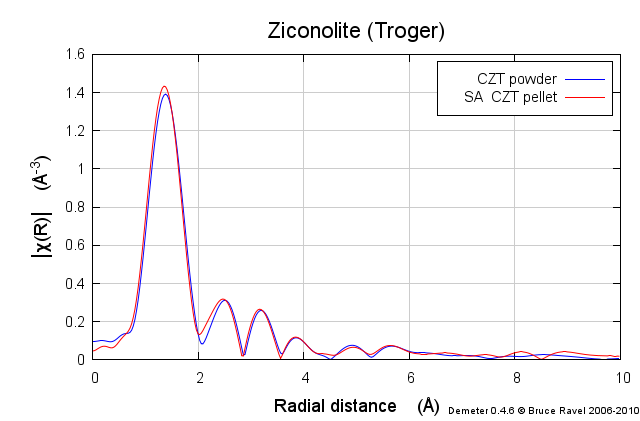
\includegraphics[width=0.8\linewidth]{images/zirconolite_chir.png}
      \end{center}
    \end{column}
  \end{columns}
\end{frame}

\begin{frame}
  \frametitle{Correct the irradiated data}
  Apply the same correction to the irradiated data measured in the same geometry.
  \begin{columns}
    \begin{column}{0.5\linewidth}
      \begin{center}
        uncorrected\\
        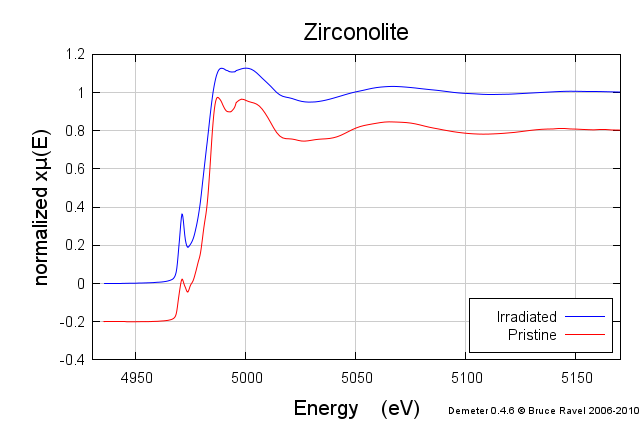
\includegraphics[width=0.8\linewidth]{images/pristine_irrad.png}
      \end{center}
    \end{column}
    \begin{column}{0.5\linewidth}
      \begin{center}
        properly corrected\\
        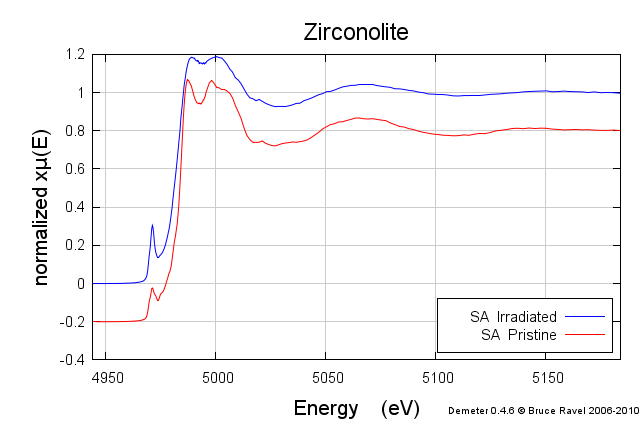
\includegraphics[width=0.8\linewidth]{images/zirconolite_fixed.png}
      \end{center}
    \end{column}
  \end{columns}

  \bigskip

  We can now apply Farge's characterization to these XANES data
  \textit{and} analyze the EXAFS data for a reasonably accurate
  coordination number.

  \medskip

  \begin{exampleblock}{}
    In this case, we had an independent metric for determining the
    proper self-absorption correction.
  \end{exampleblock}
  \begin{textblock*}{0.5\linewidth}(0pt,19.5\TPVertModule)
    \tiny%
    D.P.~Reid, et al, Nucl.\ Inst.\ Meth.\ B \textbf{268}:11-12 (2010)
    1847
    \href{http://dx.doi.org10.1016/j.nimb.2010.02.026}
    {\color{Blue2}doi:10.1016/j.nimb.2010.02.026}
  \end{textblock*}
\end{frame}

\begin{frame}
  \frametitle{Morphology}
  \begin{exampleblock}{}
    Why did I emphasize that the sample was polished a few slides back?
  \end{exampleblock}

  The glancing angle approch only works if the surface is smooth on
  the length scale of the absorption length.
  \begin{center}
    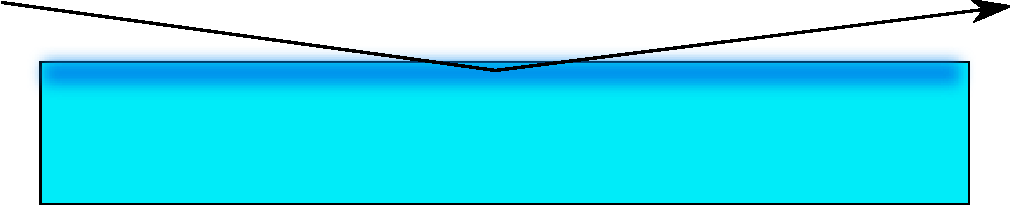
\includegraphics[width=0.8\linewidth]{images/smooth.pdf}
  \end{center}

  If the surface is rough on that length scale than individual rays
  are not guaranteed to actually hit the surface at glancing angle.
  \begin{center}
    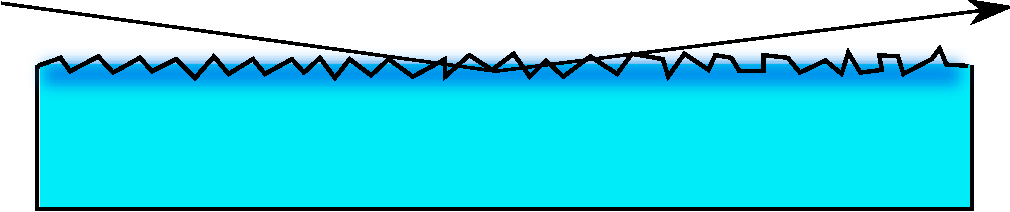
\includegraphics[width=0.8\linewidth]{images/rough.pdf}
  \end{center}


\end{frame}

\section{Conclusion}

\begin{frame}
  \frametitle{The unavoidable experiment}

  \begin{alertblock}{Oh noes!$^*$}
    Sometimes you simply cannot avoid measuring data that suffer from
    self-absorption attenuation \textbf{and} you have \textit{no way}
    of properly correcting for it.
  \end{alertblock}
  \begin{columns}
    \begin{column}{0.25\linewidth}
      
\includegraphics[width=\linewidth]{images/DontPanic.png}      
    \end{column}
    \begin{column}{0.75\linewidth}
      The standard advice applies.
      
      \medskip

      Self-absorption  is usually not a disaster.  It mostly affects
      the amplitude of $\chi(k)$ and has little to no impact on the
      phase of  $\chi(k)$.
    \end{column}
  \end{columns}

  \bigskip

  \begin{itemize}
  \item Self-absorption adds systematic uncertainty to your
    determination of coordination number and $\sigma^2$
  \item $\Delta R$ and $E_0$ can usually be measured as accurately in
    attentuated as in a tranmsission experiment.
  \end{itemize}

  \begin{textblock*}{0.5\linewidth}(0pt,19\TPVertModule)
    \tiny%
    $^*$ What to say when the giant, rhinocerous-like alien comes to eat
    you in your poorly-constructed marine base.

    \raggedleft{Urban Dictionary}
  \end{textblock*}
\end{frame}

\begin{frame}
  \frametitle{Implementation in Athena}
  \small
  {\athena} implements 4 different correction algorithms, allowing you
  to compare and contrast.

  \medskip

  \begin{description}[Tr\"oger]
  \item[Fluo] \textit{Advantage: can be applied to XANES data}\\
    Haskel, Ravel, and Stern, no reference
  \item[Tr\"oger] \textit{Simple correction to $\chi(k)$}\\L. Tr\"oger, et
    al., PRB \textbf{46}:6, (1992) 3283.
    \href{http://dx.doi.org/10.1103/PhysRevB.46.3283}{\color{Blue2}DOI:
      10.1103/PhysRevB.46.3283}
  \item[Booth] \textit{Advantage: applicable to the thin sample limit}\\
    C. H. Booth and F. Bridges, Physica Scripta, \textbf{T115}, (2005)
    202.  \href{http://dx.doi.org/10.1238/Physica.Topical.115a00202}
    {\color{Blue2}DOI:10.1238/Physica.Topical.115a00202}\\ See also
    Corwin's web site: \href{http://lise.lbl.gov/RSXAP/}
    {\color{Blue2}\texttt{http://lise.lbl.gov/RSXAP/}}
  \item[Atoms] \textit{Dead simple correction to $\chi(k)$}\\
    B. Ravel, J. Synchrotron Radiat., \textbf{8}:2, (2001) 314. 
    \href{http://dx.doi.org/10.1107/S090904950001493X}
    {\color{Blue2}DOI:10.1107/S090904950001493X}
  \end{description}
\end{frame}


\end{document}

%%% Local Variables:
%%% mode: latex
%%% TeX-master: t
%%% End:
